\begin{surferPage}[Chmutov-Ottica]{Una Ottica di Chmutov}
    Una caratteristica appariscente della ottica (superficie di grado $8$) di Chmutov $\text{Chm}_{d}, \ d=8,$ \`e la sua simmetria. Questa pu\`o anche essere vista esaminando l'equazione
    \[\text{Chm}_{d}\colon T_d(x) + T_d(y) + T_d(z) + 1 = 0,\]
     dove $T_d$ \`e il cosiddetto polinomio di Tchebychev (figura a sinistra).
    La curva $T_8(x)+T_8(y)=0$ \`e raffigurata a destra:
    
     \begin{center}
      \begin{tabular}{c@{\quad}c}
        \begin{tabular}{c}
          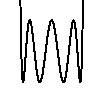
\includegraphics[height=1.75cm]{Tcheb_008.pdf}
        \end{tabular}    
        &
        \begin{tabular}{c}
          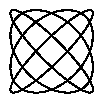
\includegraphics[height=1.75cm]{Tcheb_2d_008.pdf}
        \end{tabular}    
      \end{tabular}
    \end{center}
    \vspace{-0.3cm}
    I passi necessari per andare da queste figure alla forma della superficie nel visore interattivo non sono molto difficili.

Queste equazioni furono date da S.V.\ Chmutov nei primi anni Ottanta. Al tempo, esse costituivano il record mondiale per $\mu(d)$ per la maggior parte dei $d$. Negli anni Novanta, Chmutov miglior\`o il suo stesso record, e nel 2005 S.~Breske, O.~Labs e D.~van~Straten adattarono questa costruzione per produrre superfici reali con solo singolarit\`a reali.
\end{surferPage}